\documentclass[twocolumn]{article}
\usepackage[utf8]{inputenc}
\usepackage[spanish]{babel}
\usepackage{hyperref}
\usepackage{graphicx}
\graphicspath{ {img/} }

\title{\textbf{Reporte del primer proyecto}}
\author{José Alonso Landín Rangel}
\date{17 de junio del 2021}

\begin{document}

\maketitle

\begin{abstract}
    Se realizó una regresión lineal sobre los datos de las lista nominal por cada municipio del estado de Guanajuato, con el fin de obtener una estimación del número de casillas necesarias a instalar por municipio si la jornada electoral hubiese sido el 28 de febrero del 2021.
\end{abstract}

\section{Fuentes de datos}

Se utilizaron los datos abierto del Instituto Nacional Electoral (INE), disponibles para su descarga en \cite{INE}. Se usaron solamente los archivos de enero a diciembre del 2020.

\medskip

\section{Procedimiento y resultados}


Primeramente, se realizó el filtrado de los datos para seleccionar sólo los correspondientes al estado de Guanajuato. Después, se realizó una regresión lineal sobre el total de la lista nominal por municipio, en base a la cual se extrapoló una proyección para la misma al 28 de febrero del 2021.

\medskip

En base a esta proyección, se calculó el incremento porcentual esperado en la lista nominal por municipio
entre enero del 2020 y febrero del 2021; esta tasa 
de incremento fue aplicada después a la lista nominal de cada sección electoral en el estado en 
enero del 2020, obteniéndose así un estimado de la lista nominal por sección en esta fecha.

\medskip

Con la estimación de la lista nominal por sección, se determinó el número de casillas 
necesarias para garantizar el voto a la totalidad de los ciudadanos inscritos en la misma, 
sabiendo que cada casilla tendrá a su disposición 750 boletas electorales. Los resultados se muestran en la tabla \ref{tab:1}.

\begin{table}[p]
\begin{center}
    \begin{tabular}{|c|c|}
    \hline
        Municipio & Casillas estimadas \\
    \hline
     1 & 234\\
     2&175\\
     3&227\\
     4&92\\
     5&115\\
     6&8\\
     7&646\\
     8&65\\
     9&105\\
     10&18\\
     11&131\\
     12&43\\
     13&32\\
     14&190\\
     15&238\\
     16&30\\
     17&707\\
     18&51\\
     19&82\\
     20&1921\\
     21&77\\
     22&36\\
     23&232\\
     24&19\\
     25&89\\
     26&88\\
     27&368\\
     28&158\\
     29&52\\
     30&149\\
     31&160\\
     32&102\\
     33&152\\
     34&9\\
     35&102\\
     36&13\\
     37&226\\
     38&20\\
     39&60\\
     40&25\\
     41&83\\
     42&195\\
     43&28\\
     44&80\\
     45&19\\
     46&112\\
     \hline
    \end{tabular}
\end{center}
\caption{Casillas estimadas por municipio}
\label{tab:1}
\end{table}

Estos resultados son ligeramente distintos a los obtenidos con el análisis anterior usando Excel, que se muestran para su comparación en la tabla de la figura \ref{fig:1}.

\begin{figure}[p]
    \centering
    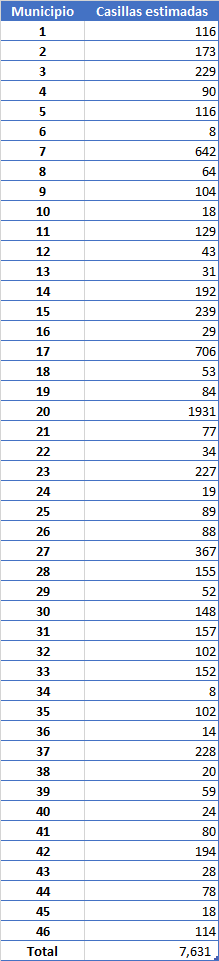
\includegraphics[scale=0.7]{Casillas.png}
    \caption{Resultados usando datos desde marzo del 2019}
    \label{fig:1}
\end{figure}

\begin{thebibliography}{9}
\bibitem{INE}
Instituto Nacional Electoral (INE)
\textit{Estadística de Padrón 
Electoral y Lista Nominal de Electores}
31/12/2020. Disponible en: \url{https://www.ine.mx/transparencia/datos-abiertos/#/archivo/estadistica-padron-electoral-lista-nominal-electores}
\end{thebibliography}
\end{document}
